\documentclass[a4paper,10pt,notitlepage]{article}

\usepackage[]{geometry}
\usepackage{setspace, soul}
\usepackage{psfrag}
\usepackage[dvips]{graphicx}
\usepackage{pstricks}
\usepackage[document]{ragged2e}
\usepackage{acronym}
\usepackage{latexsym}

\usepackage{amsthm}
\usepackage{amsmath}
\usepackage{wrapfig}
\usepackage{lipsum}
\usepackage{hyperref}
\usepackage{enumitem}
\usepackage[utf8]{inputenc}
%\usepackage[utf8]{vietnam}
\usepackage{graphicx}
\usepackage[hidelinks]{hyperref,xcolor}
\usepackage{fancyheadings}

\usepackage{setspace,subfigure}
\usepackage{titlesec}
\usepackage{xcolor}
\usepackage[colorlinks=true,linkcolor=udc]{hyperref}
%\usepackage{helvet}
\usepackage{array,amssymb,amsthm,amsmath,amstext}
\usepackage{afterpage}
\usepackage[font=small,bf]{caption}
\usepackage{colortbl}
\usepackage{emptypage}
\usepackage{listings} 
\usepackage{lscape}
\usepackage{array}
\usepackage{tikz} 


\usepackage{amsmath}
\usepackage{unicode-math}
\usepackage[T1]{fontenc}
\usepackage[utf8]{inputenc}
\usepackage{xcolor}
\definecolor{textblue}{rgb}{.2,.2,.7}
\definecolor{textred}{rgb}{0.54,0,0}
\definecolor{textgreen}{rgb}{0,0.43,0}
\usepackage{listings}
\lstset{language=Python, 
numbers=left, 
numberstyle=\tiny, 
stepnumber=1,
numbersep=5pt, 
tabsize=4,
basicstyle=\ttfamily,
keywordstyle=\color{textblue},
commentstyle=\color{textgreen},   
stringstyle=\color{textred},
frame=none,                    
columns=fullflexible,
keepspaces=true,
xleftmargin=\parindent,
showstringspaces=false}

%%%%%%%%%%%%%%%%%%%%%%%%%%%%%%%%%%%%%%%%%%%%%%%%%%%%%%%%%%%%%%%%%%%%%%%%%%%%%%%%%%%%%%%%%%%%%%%%%%%%%%%%%%%%%%%%%%%%%%
\usepackage{background}
\backgroundsetup{contents=
\includegraphics{hustlogo.png}, scale = 0.45, angle = 0, opacity=0.25}

\definecolor{udc}{rgb}{0.58,0.0.01,0.04} 

\pagestyle{fancy}
\renewcommand{\headrulewidth}{0pt}
\renewcommand\UrlFont{\color{blue}\rmfamily}
% set page geometry
\geometry{a4paper, total={140mm,250mm}, left=20mm, right=20mm, top=14mm, bottom=30mm}

\title{Diffusion-Limited Aggregation model}
\author{{Vu Duc An 20215174}
\\ {Le Ha Ngan 20215230}
\\ {Dang Viet Hoang 20215206}
\\ {Trinh Diem Quynh 20210737}
\\ {Trinh Thi Dieu Thuy 20215247}}
\newcommand{\mails}{ {an.vd215174@sis.hust.edu.vn}
\\ {ngan.lh215230@sis.hust.edu.vn}
\\ {hoang.dv215206@sis.hust.edu.vn}
\\ {quynh.td210737@sis.hust.edu.vn}
\\ {thuy.ttd215247@sis.hust.edu.vn}}
\newcommand{\class}{727616 - IT4110E}
\newcommand{\lecturer}{{Vu Van Thieu}
\\thieu.vuvan@hust.edu.vn
}

\date{\today}
\makeatletter{}

\usepackage{biblatex}
\addbibresource{citations.bib}

\begin{document} \raggedright
%%%%%%%%%%%%%%%%%%%%%%%%%%%%%%%%%%%%%%%%%%%%%%%%%%%%%%%%%%%%%%%%%%%%%%%%%%%%%%%%%%%%%%%%%%%%%%%%%%%%%%%%%%%%%%%%%%%%%%%%%%%%%%%%%%
\NoBgThispage
\thispagestyle{empty}

	\newcommand{\HRule}{\rule{\linewidth}{0.3mm}} 
	\center 
	\MakeUppercase{\large Hanoi University of Science and Technology
	\\ \LARGE School of Information and Communication Technology}\\[0.5cm]
		{
\includegraphics[width=0.25\textwidth]{hustlogo.png} \par}\\[0.5cm]
	\textsc	{\MakeUppercase{\Large Scientific Computing project report}\\[0.75cm]}
	
	\textsc	{\MakeUppercase{\large Scientific Computing\\\normalsize (IT4110E)}\\[0.5cm]}
	
	\HRule\\[0.4cm]

	{\huge\bfseries \@title}\\[0.4cm]
	
	\HRule\\[1.5cm]
	\begin{minipage}{0.4\textwidth}
		\begin{flushleft}
			\large
			\textit{Team members}\\
			\@author
		\end{flushleft}
	\end{minipage}
	~
	\begin{minipage}{0.4\textwidth}
		\begin{flushright}
			\large
			\textit{Email}\\
			\mails 
		\end{flushright}
	\end{minipage}
\vfill\vfill
        \begin{minipage}{0.4\textwidth}
		\begin{center}
			\large
			\textit{Class}\\
			\class\\
			\textit{Lecturer}\\
			\lecturer\\
		\end{center}
	\end{minipage}
\vfill\vfill
		{\large\today} 
    \vfill\vfill
    \normalsize{Time period: $23^{nd}$June - $7^{th}$July}
    \\[0.3cm]
   
    \homepage
    
    \vfill
    
%\input{./title.tex}
%%%%%%%%%%%%%%%%%%%%%%%%%%%%%%%%%%%%%%%%%%%%%%%%%%%%%%%%%%%%%%%%%%%%%%%%%%%%%%%%%%%%%%%%%%%%%%%%%%%%%%%%%%%%%%%%%%%%%%%%%%%%%%%%%%%%%%
\newpage
\centering
% \thispagestyle{empty}
\pagestyle{plain}
\thispagestyle{empty}
\backgroundsetup{contents = 
\includegraphics{soictlogo.png}, scale = 0.5, vshift = 5cm, angle = 50, opacity = 0.05}
\begin{center}
   \large \textbf{Scientific Computing Report\\}
   \normalsize \textbf{Diffusion-Limited Aggregation model\\}
   \small
   Class: 727616\\
   Lecturer: Vu Van Thieu\\
    
\end{center}
\large
\tableofcontents

%%%%%%%%%%%%%%%%%%%%%%%%%%%%%%%%%%%%%%%%%%%%%%%%%%%%%%%%%%%%%%%%%%%%%%%%%%%%%%%%%%%%%%%%%%%%%%%%%%%%%%%%%%%%%%%%%%%%%%%%%%%%%%%%%%%
\newpage
\backgroundsetup{contents = 
\includegraphics{soictlogo.png}, scale = 0.5, vshift = 5cm, angle = 50, opacity = 0.05}
\renewcommand{\thesection}{\Roman{section}} 
%\renewcommand{\thesubsection}{\Roman{subsection}}
\pagestyle{plain}
\raggedright

\setlength{\parindent}{1cm}

\section{\textbf{Introduction}}
    % \begin{figure}[h]
    %     \centering
    %     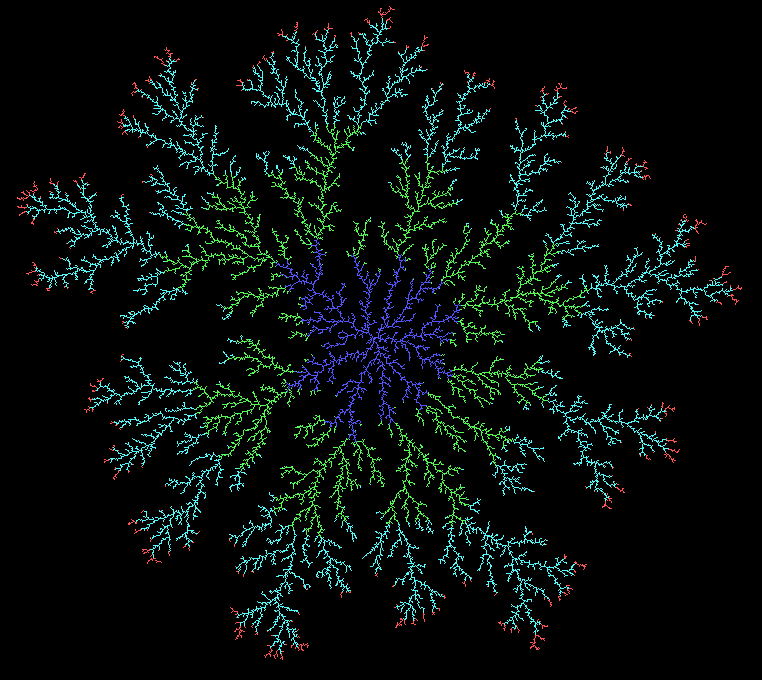
\includegraphics[width = 7cm]{Of7_p0001_15h.jpg}
    % \end{figure}
{\setlength{\parskip}{0.5cm}
\vspace{-0.5cm}
\hspace{1 cm}
\subsection{Diffusion-Limited Aggregation}
\hspace{1 cm}The Diffusion-Limited Aggregation (DLA) problem is a mathematical problem that involves simulating the growth of a random cluster of particles that are randomly moving in space and sticking together when they come into contact with each other. \\
In this context, DLA is often used to model the growth and aggregation of various entities, such as particles, cells, or organisms.
\subsection{Real-world applications:}
\hspace{1 cm}The DLA problem has practical applications in various fields such as physics, chemistry, biology and computer science. It is commonly used to simulate the growth and development of living organisms, including viruses, algae, and cells. Additionally, DLA can be applied to understand and describe physical processes such as dissolution and permeation. By studying DLA, researchers can gain insights into the dynamics and patterns of growth in complex systems.
\subsection{Problem statement:}
\hspace{1 cm}In the scope of this report, we focus on simulating the growth of virus entities within a limited environment that contains a food source. The objective is to model how the viruses interact with their surroundings, consume food, and undergo continuous growth. By analyzing the simulated growth patterns, we aim to gain a better understanding of the dynamics and behavior of virus populations in confined environments. This information can have implications in various fields, including biology, epidemiology, and materials science.
\newpage
\section{\textbf{Theory}}
\subsection{Theorem statement:}
{\setlength{\parskip}{0.5cm}
\label{sec:TS}
\hspace{1 cm}During the description process, bacteria will grow from an initial cell. The growth of bacteria in the food environment is probabilistic and depends on the food concentration in the surrounding cells.

The food concentration in the environment is continuously changing, and cells containing bacteria will deplete the available food. The difference in food availability will be influenced by the diffusion equation.

The diffusion equation simulates the changes in food concentration, which occur much faster compared to the growth rate of the virus. Therefore, the diffusion process can be considered instantaneous, and a time-independent diffusion equation will be used to determine the food concentration.
\begin{eqnarray} 
    \frac{\partial c}{\partial t} = D\bigtriangledown^2c
\end{eqnarray}
\normalsize
					\hspace{8cm}\textbf{D:} Diffusion coefficient.\\
					\hspace{7cm}\textbf{C:} Concentration.\\
\large
Since the equation is time-independent, the derivative of the concentration with respect to time can be considered as zero.

The above equation can be solved directly or using iterative methods. The Successive Over Relaxation (SOR) method will be presented in the following section of the report.
\subsection{SOR method:}
{\setlength{\parskip}{0.5cm}
\vspace{-0.5cm}
\hspace{1 cm}The Successive Over Relaxation (SOR) method uses the following formula to calculate Ci,j:
\begin{eqnarray}
    c^{k+1}_{i, j} = \frac{\omega}{4} \left( c^{(k)}_{i+1, j} + c^{(k+1)}_{i-1, j} + c^{(k)}_{i, j+1} + c^{(k+1)}_{i, j-1} \right) + (1-\omega)c^{k}_{i, j}
\end{eqnarray}
\hspace{1 cm}Where $\omega$ is the relaxation parameter. The parameter $\omega$ indicates how much the concentration at a position in the previous iteration influences the next iteration. In the SOR method, we use a value of $\omega$ within the range of $(1, 2)$.

Specifically, in this report, we will investigate the SOR method with a value of $\omega=1.89$.
\subsection{Application to the DLA problem:}
    The basic algorithm for simulating the DLA process is as follows:
    \begin{enumerate}
        \item Solve the diffusion equation to obtain the food concentration matrix.
        \item Allow viruses to reproduce (according to probabilities).
        \item Repeat steps 1 and 2.
    \end{enumerate}
    Specifically:\\
    Step 1: The concentration matrix is generated using the SOR method.\\
Step 2: Each neighboring cell of a virus has a probability of being infected, which is proportional to the food concentration in that cell.\\
\vspace{0.5cm}
    \begin{figure}[h]
        \centering
        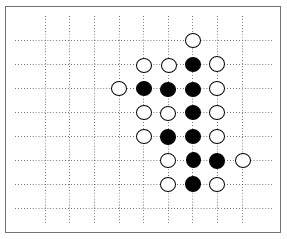
\includegraphics[width = 7cm]{img2.3.png}
    \end{figure}

    The image above illustrates a stage in the virus development process. The black cells represent infected cells, while
    the white cells represent potential sites for further virus growth.
The probability of virus growth in each white cell is calculated using the equation:
\begin{eqnarray}
    P_g((i,j) \in \circ \rightarrow (i,j)\in \bullet) = \frac{(c_{i,j})^\eta}{\displaystyle\sum_{(i,j)\in\circ}(c_{i,j})^\eta}
\end{eqnarray}

Where the exponent $\eta$ determines the shape of the virus cluster and is typically chosen between 0.5 and 2.
In this report, different values of $\eta$ will be investigated.

\newpage
\section{\textbf{Implementation: }}
{\setlength{\parskip}{0.5cm}
\vspace{1.5cm}
\begin{lstlisting}
import numpy as np

# Size of the grid: size
# Exponent p (eta) - in the probability formula
# Place the first virus at position x_start, y_start
def simulate(size, p, x_start, y_start):
    temp_values = []

    n = 4000 # Number of viruses
    nVirus = 1

    # Food concentration array
    C = np.zeros((size, size))
    temp = np.zeros((size, size))

    # Setting omega parameter
    w = 1.89

    # Grow array marks  locations where the viruses grow
    grow = np.zeros((size, size))
    grow[x_start, y_start] = 1

    # Setting default food
    for i in range(1, size - 1):
        for j in range(1, size - 1):
            C[i, j] = 1

    C[x_start, y_start] = 0

    while True:
        candidate = np.zeros((size, size))
        sumOfChance = 0
                
        # SOR method to calculate at step k+1
        for i in range(1, size - 1):
            for j in range(1, size - 1):
                if C[i, j] != 0:
                    C[i, j] = (w/4) * (C[i+1, j] + C[i-1, j] 
                    + C[i, j+1] + C[i, j-1]) + (1-w) * C[i, j]

                if C[i, j] < 0:
                    temp[i, j] = 0
                else:
                    temp[i, j] = C[i, j]

        # Find candidates
        for i in range(1, size - 1): 
            for j in range(1, size - 1):
                if grow[i, j] == 1:
                    C[i, j] = 0
                    if grow[i-1, j] == 0 and candidate[i-1, j] == 0:
                        candidate[i-1, j] = 1
                    if grow[i+1, j] == 0 and candidate[i+1, j] == 0:
                        candidate[i+1, j] = 1
                    if grow[i, j-1] == 0 and candidate[i, j-1] == 0:
                        candidate[i, j-1] = 1
                    if grow[i, j+1] == 0 and candidate[i, j+1] == 0:
                        candidate[i, j+1] = 1

        # Calculate the denominator of P
        for i in range(1, size - 1):
            for j in range(1, size - 1):
                if candidate[i, j] == 1:
                    sumOfChance += C[i, j]**p

        # Random grow
        for i in range(1, size - 1):
            for j in range(1, size - 1):
                if candidate[i, j] == 1:
                    randPos = np.random.rand() / 10
                    curChance = (C[i, j]**p) / sumOfChance
                    if randPos < curChance:
                        grow[i, j] = 1
                        if nVirus < 4000:
                            nVirus += 1
                            
        temp_values.append(temp.copy())
        print(nVirus, end="\r")
        
        if nVirus == 4000:
            return temp_values
            break

import matplotlib.pyplot as plt
from mpl_toolkits.mplot3d import Axes3D
        
def run_sim(size = 201, p = 2, x_start = 2, y_start = 100, name = ''):
    filename = '{0}x{0}p{1}plot{2}'.format(size-1, p, name)
    try:
        # Load the array from the file if exist
        temp_values = np.load('data/' + filename + '.npy')
    except FileNotFoundError:
        temp_values = simulate(size, p, x_start, y_start)
        np.save('data/' + filename + '.npy', temp_values)

    temp = temp_values[-1]
    
    x = np.arange(size)
    y = np.arange(size)
    X, Y = np.meshgrid(x, y)

    fig, (ax, ax_top) = plt.subplots(1, 2, figsize=(10, 5)
                        , subplot_kw={'projection': '3d'})
    ax.plot_surface(X, Y, temp, cmap='jet')
    ax.view_init(azim=-120, elev=30)
    
    ax_top.contourf(X, Y, temp, cmap='jet')
    ax_top.view_init(azim=-90, elev=90)
    ax_top.set_zticks([])
    
    plt.savefig(filename + '.png', transparent=True)
    plt.show(block=False)
    
# Make directory
import os
path = "data"
# Check whether the specified path exists or not
isExist = os.path.exists(path)
if not isExist:
   os.makedirs(path)
\end{lstlisting}
\vspace{1.5cm}

Program used Python, and libary matplotlib, mpltoolkits to get result images.
To run the program, use command \texttt{run\_sim} with arguments:

\texttt{p} : Value of exponent $\eta$

\texttt{size} : The size of simulation

\texttt{x\_start, y\_start} : Starting position of the virus

\texttt{name} : Additional string to append to the output image file

For example, run one of the following:
\begin{lstlisting}
run_sim(p = 0)
run_sim(size = 201, p = 1)
run_sim(size = 501, p = 2, x_start = 2, y_start = 100, name = '-mid')
\end{lstlisting}

\newpage
\subsection{Data structure:}
    \vspace{-0.8cm}
    \hspace{1 cm}

2D \texttt{\textbf{Numpy}} array \texttt{candidate[][]} contains a list of candidates that can be infected with the virus in the current step

\texttt{C[][]} array represents the remaining food in the area, initialized to 1, except for a single cell containing the first virus

The \texttt{grow[][]} array is used to mark the position of the viruses.

\subsection {Program structure:}
    \vspace{-0.5cm}
    \hspace{1 cm}
\begin{enumerate}
        \item Initialize \texttt{C[][]} equal 1 (because have no virus eat food ), \texttt{grow[][]}, \texttt{candidate[][]} equal 0 
        \item Perform the SOR iteration method to calculate the entire \texttt{C[][]} matrix.
        \item Find candidates place where having growth of viruss
        \item Randomly generate viruses
        \item Loop untill find enough viruss 
    \end{enumerate}
\vspace{0.5cm}
\subsection{Graph plotting:}
    \vspace{-0.5cm}
    \hspace{1 cm} 
    The result matrix is stored in the file and gif.
This will create a visualization of the matrix using colors to represent different values.
}
\vspace{1.5 cm}
\section{\textbf{Experimental results:}}
{\setlength{\parskip}{0.5cm}
    \vspace{0.5cm}
    \hspace{1 cm}
    We release the first virus at the bottom of the screen and run simulations with different sizes:
The redder the position, the higher the food concentration. Light red or yellow positions indicate areas with less food, while the darkest blue indicates the presence of viruses.
\newpage
Running with a size of \textbf{200x200}, producing \textbf{4,000} viruses.

\begin{itemize}
    \item With $\eta=0$:
    \begin{figure}[h]
        \centering
        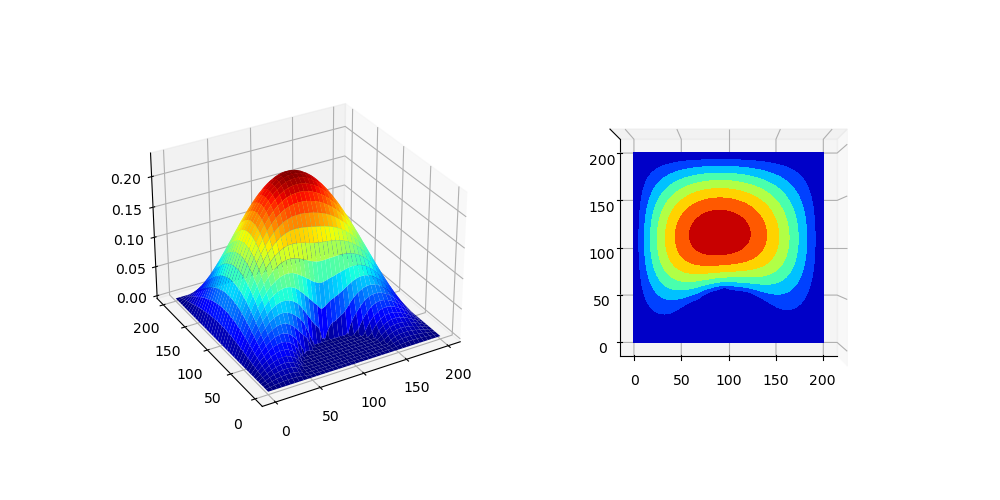
\includegraphics[trim=70pt 40pt 100pt 60pt, clip, height = 6cm]{200x200p0plot.png}
    \end{figure}
    \item  With $\eta = 1$:
    \begin{figure}[h]
        \centering
        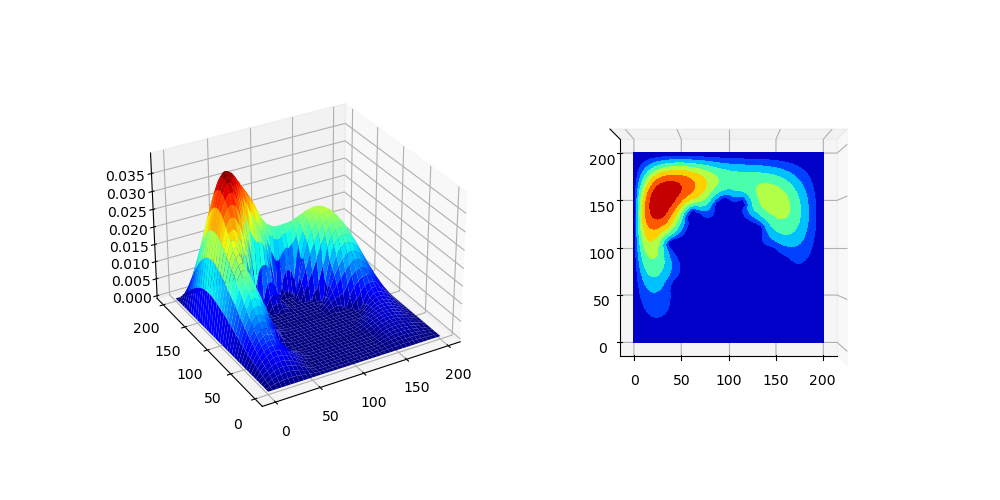
\includegraphics[trim=70pt 40pt 100pt 60pt, clip, height = 6cm]{200x200p1plot.png}
    \end{figure}
    \item  With $\eta = 2$:
    \begin{figure}[h]
        \centering
        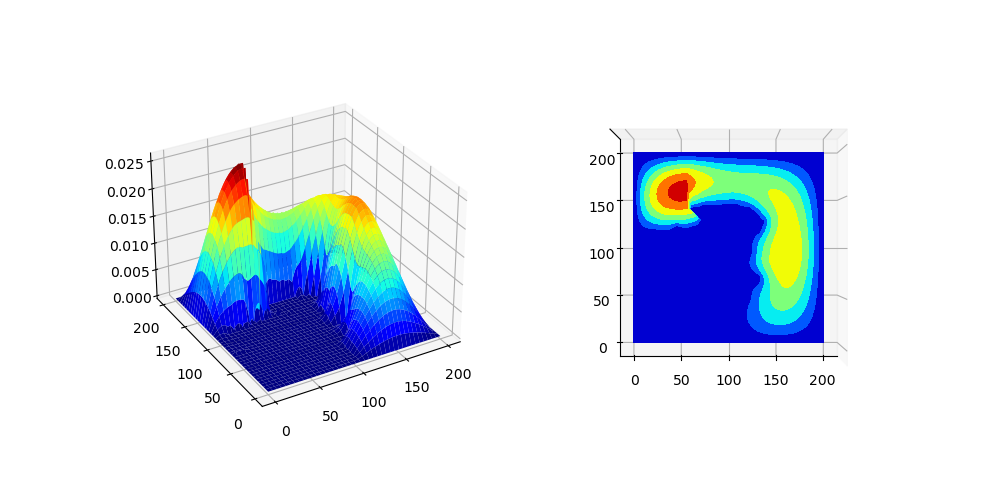
\includegraphics[trim=70pt 40pt 100pt 60pt, clip, height = 6cm]{200x200p2plot.png}
    \end{figure}
\end{itemize}
\newpage
Running with a size of \textbf{500x500}:
\begin{itemize}
    \item With $\eta = 0$:
    \begin{figure}[h]
        \centering
        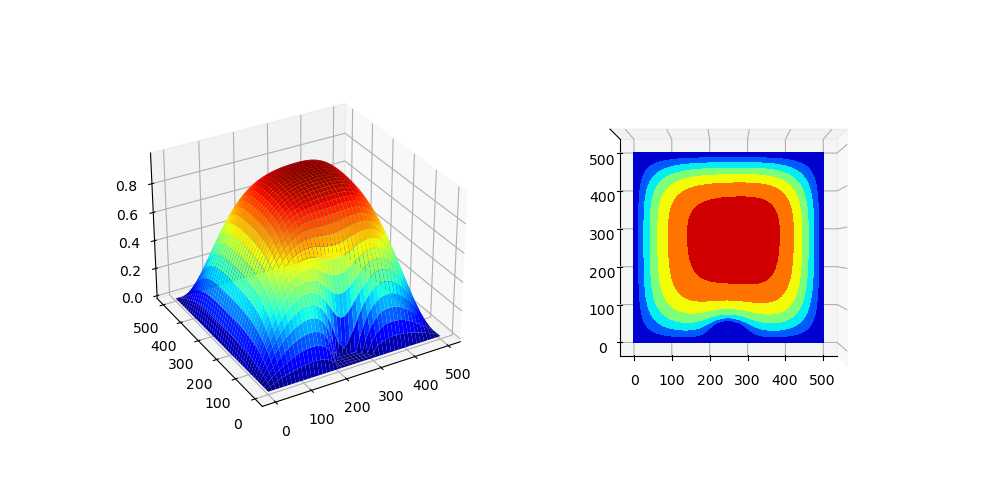
\includegraphics[trim=70pt 40pt 100pt 60pt, clip, height = 6cm]{500x500p0plot.png}
    \end{figure}
    \item  With $\eta = 1$:
    \begin{figure}[h]
        \centering
        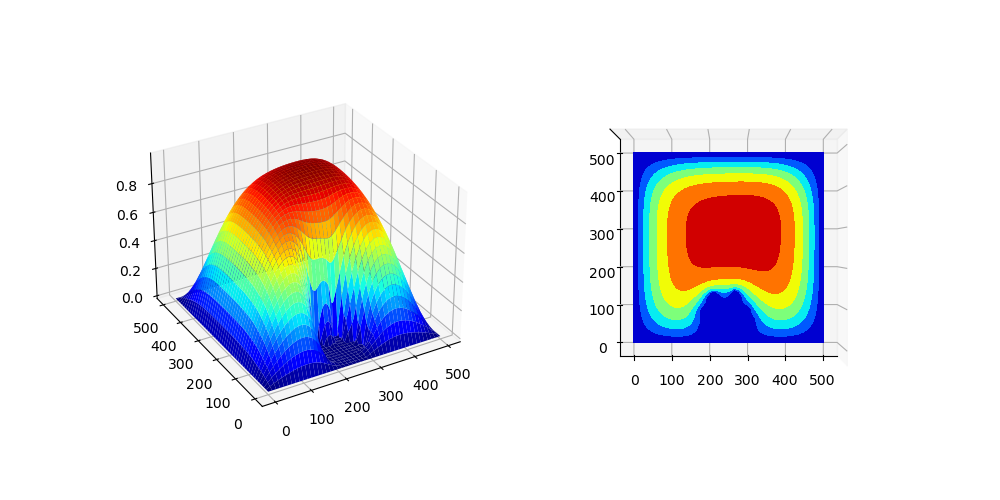
\includegraphics[trim=70pt 40pt 100pt 60pt, clip, height = 6cm]{500x500p1plot.png}
    \end{figure}
    \item  With $\eta = 2$:
    \begin{figure}[h]
        \centering
        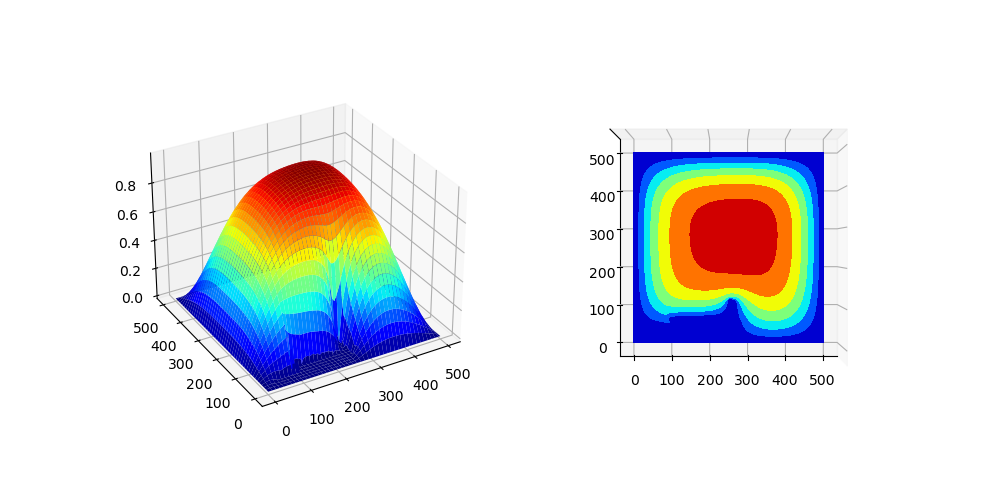
\includegraphics[trim=70pt 40pt 100pt 60pt, clip, height = 6cm]{500x500p2plot.png}
    \end{figure}
\end{itemize}
\newpage
Similarly, but with viruses growing from the center of the screen:
\begin{itemize}
    \item With $\eta = 0$:
    \begin{figure}[h]
        \centering
        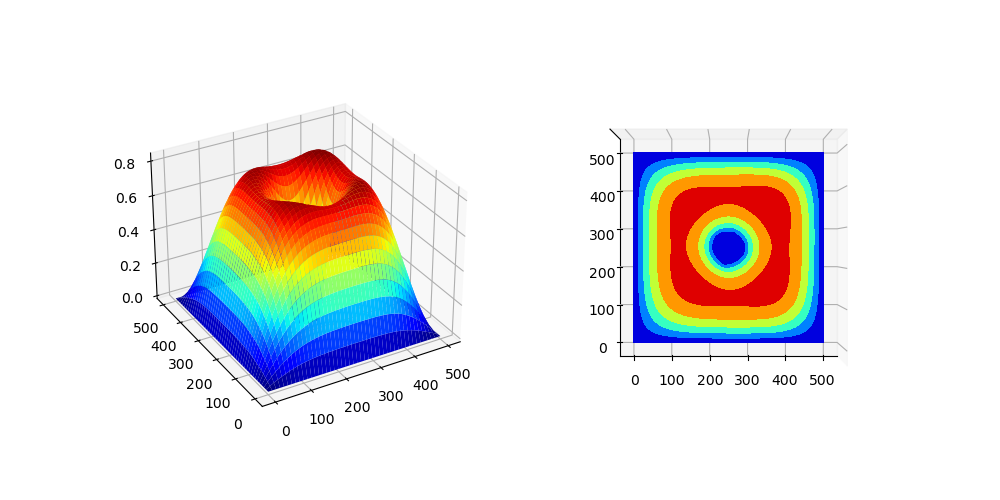
\includegraphics[trim=70pt 40pt 100pt 60pt, clip, height = 6cm]{500x500p0plot-mid.png}
    \end{figure}
    \item  With $\eta = 1$:
    \begin{figure}[h]
        \centering
        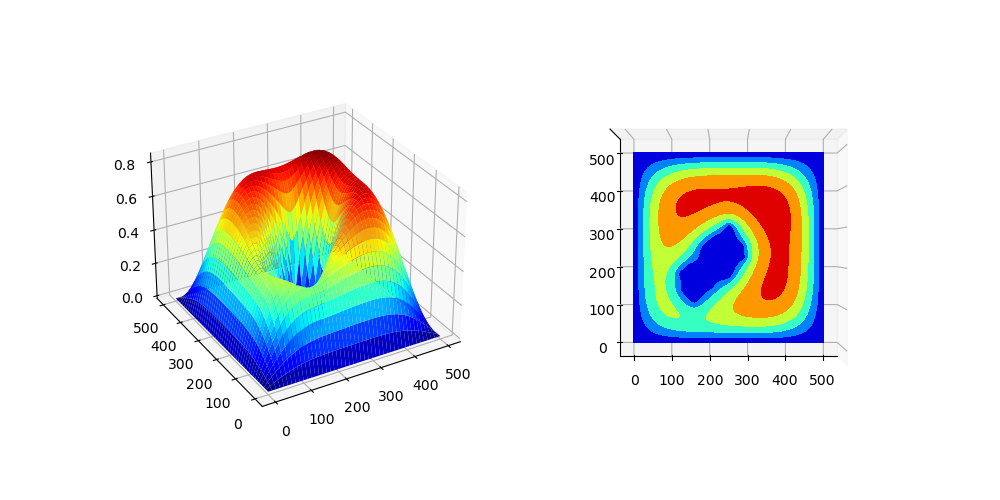
\includegraphics[trim=70pt 40pt 100pt 60pt, clip, height = 6cm]{500x500p1plot-mid.png}
    \end{figure}
    \item  With $\eta = 2$:
    \begin{figure}[h]
        \centering
        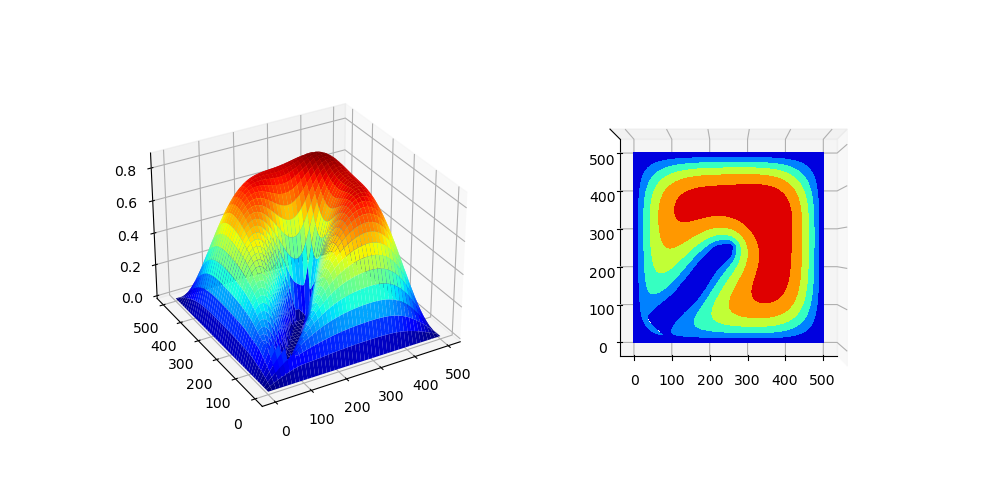
\includegraphics[trim=70pt 40pt 100pt 60pt, clip, height = 6cm]{500x500p2plot-mid.png}
    \end{figure}
\end{itemize}
\newpage
\textbf{Observations:}\\
The exponent $\eta$ affects the virus growth pattern.
With $\eta = 0$, the probability of new virus appearance is the same everywhere, resulting in a symmetrical pattern.
With $\eta = 1$, the probability of new virus appearance is proportional to the available food concentration, which is reasonable in nature. The pattern typically exhibits a few branching structures.\\
With $\eta = 2$, the probability is proportional to the square of the food concentration. Regions with higher food concentration have a significantly higher probability of new virus appearance. Consequently, the virus growth pattern exhibits fewer branching structures.
}
\section{\textbf{Conclusion:}}
The report provides an overview of the principles and algorithms used in the DLA simulation method. It discusses the concepts of diffusion-limited aggregation and its applications in various fields. The theoretical aspects, including the theorem statement and the SOR method, are explained in detail. The implementation section covers the data structure, program structure, and graph plotting techniques employed in the simulation. The report concludes with the experimental results obtained from running the simulation and provides evaluations and conclusions drawn by the team based on these results.





\section{\textbf{Reference}}
\nocite{*}
\printbibliography

\newpage %%%%%%%%%%%%%%%%%%%%%%%%%%%%%%%%%%%%%%%%%%%%%%%%%%%%%%%%%%%%%%%%%%%%%%%%%%%%%%%%%%%%%%%%%%%%%%%%%%%%%%%%%%%%%%%%%%%%%%%%%%%%%


\end{document}
